\documentclass[tikz,border=2pt]{standalone}
\usepackage{amsmath,amssymb}
\usepackage{pgfplots}
\pgfplotsset{compat=1.18}
\usetikzlibrary{arrows.meta}

\begin{document}
% y = x^2 (convex, blue) lies below its chord between x = -1.5 and x = 1.5;
% y = -x^2 (concave, red) lies above its chord.
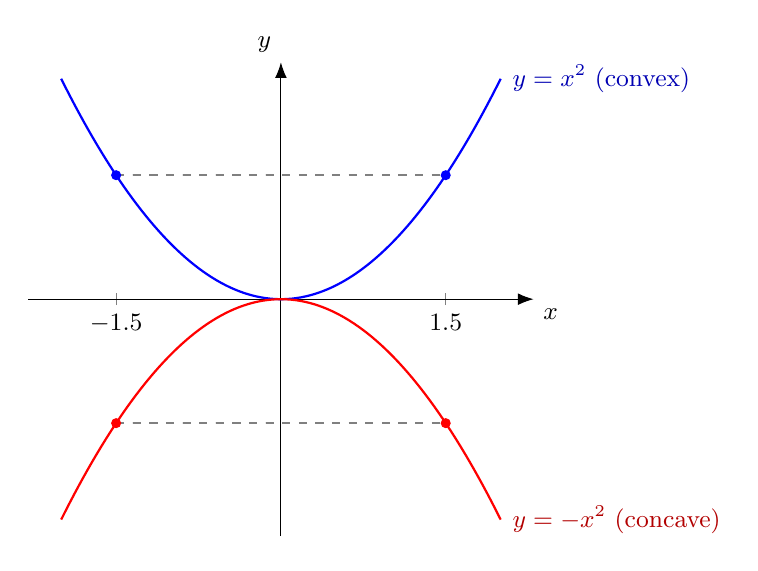
\begin{tikzpicture}[every node/.style={font=\small}]
	\begin{axis}[
		width=8cm, height=7.6cm,
		axis lines=middle, axis line style={-{Latex[length=2mm]}},
		xmin=-2.3, xmax=2.3, ymin=-4.3, ymax=4.3,
		xtick={-1.5,1.5}, ytick=\empty,
		tick label style={font=\small},
		xlabel={$x$}, ylabel={$y$},
		xlabel style={below right}, ylabel style={above left},
		samples=100, clip=false
		]
		\addplot[blue, thick, domain=-2:2] {x^2};
		\addplot[red, thick, domain=-2:2] {-x^2};
		\addplot[gray, dashed, thick, domain=-1.5:1.5] {2.25};
		\addplot[gray, dashed, thick, domain=-1.5:1.5] {-2.25};
		\addplot[only marks, mark=*, mark size=1.6pt, blue] coordinates {(-1.5,2.25) (1.5,2.25)};
		\addplot[only marks, mark=*, mark size=1.6pt, red] coordinates {(-1.5,-2.25) (1.5,-2.25)};
		\node[blue!70!black, anchor=west] at (axis cs:2.02,4) {$y=x^2$ (convex)};
		\node[red!70!black, anchor=west] at (axis cs:2.02,-4) {$y=-x^2$ (concave)};
	\end{axis}
\end{tikzpicture}
\end{document}
